\documentclass{scrartcl}

\usepackage{graphicx}
\usepackage[utf8]{inputenc}
\usepackage[T1]{fontenc}
\usepackage{lmodern}
\usepackage[english]{babel}
\usepackage{amsmath}
\usepackage{amsthm}
\usepackage{mathtools}
\usepackage{amssymb}
\usepackage{listings}
\usepackage{xparse}
\usepackage{stmaryrd}
\usepackage{geometry}
\usepackage{enumerate}
\usepackage{tikz}
\usepackage{stmaryrd}
\usepackage[style=english]{csquotes}
\usepackage[language=english, backend=biber, style=alphabetic, sorting=nyt]{biblatex}

\usetikzlibrary{babel, positioning, shapes.geometric, arrows, arrows.meta}
\addbibresource{../bibliography.bib}
\title{Generating supersingular curves with modular polynomials}
\author{Simon Pohmann}

\newcommand{\Z}{\mathbb{Z}}
\newcommand{\Q}{\mathbb{Q}}
\newcommand{\F}{\mathbb{F}}
\newcommand{\C}{\mathbb{C}}
\newcommand{\End}{\mathrm{End}}
\newcommand{\Quot}{\mathrm{Quot}}
\newcommand{\Half}{\mathcal{H}}
\newcommand{\Lattice}{\mathcal{L}}
\newcommand{\divides}{\ \mid \ }
\newcommand{\notdivides}{\ \nmid \ }
\newcommand{\Cl}{\mathrm{Cl}}
\newcommand{\q}{\mathfrak{q}}
\newcommand{\Norm}{\mathfrak{N}}
\newcommand{\IdPoint}{O}
\renewcommand{\l}{\mathfrak{l}}
\renewcommand{\a}{\mathfrak{a}}
\newcommand{\p}{\mathfrak{p}}
\renewcommand{\b}{\mathfrak{b}}
\newcommand{\val}{v}
\newcommand{\Ell}{\mathrm{Ell}}
\renewcommand{\O}{\mathcal{O}}

\newcommand\restr[2]{{
    \left.\kern-\nulldelimiterspace
    #1
    \vphantom{\big|}
    \right|_{#2}
}}

\newtheorem{prop}{Proposition}[section]
\newtheorem{theorem}[prop]{Theorem}
\newtheorem{lemma}[prop]{Lemma}
\newtheorem{corollary}[prop]{Corollary}

\theoremstyle{definition}
\newtheorem{problem}[prop]{Problem}
\newtheorem{alg}[prop]{Algorithm}
\newtheorem{definition}[prop]{Definition}
\newtheorem{example}[prop]{Example}
\newtheorem{remark}[prop]{Remark}

\begin{document}

\maketitle

\section{Introduction}

\section{Ordinary isogeny graphs}

\subsection{Imaginary quadratic orders}
For this part, let $\O$ be an order in an imaginary quadratic number field $K$.
\begin{lemma}
    Let $\p \leq \O_K$ be a prime with $\Norm(\p) \perp [\O_K : \O]$.
    Then $\p$ has a set of generators in $\O$.
\end{lemma}
\begin{proof}
    Suppose $\p$ is a prime over $p$, and let $\O = \Z[\phi]$.
    We use the decomposition law in Dedekind ring extensions.
    Since $\Norm(\p) \perp [\O_K : \O]$ are coprime, we can apply it with a generator $\phi$ of $\O$.

    If $\mathrm{MiPo}(\phi) = f(X)g(X) \mod p$ splits, then have
    \begin{equation*}
        p\O_K = (p, f(\phi))(p, g(\phi))
    \end{equation*}
    and so the prime ideals over $p$ are $(p, f(\phi))$ and $(p, g(\phi))$.
    If $\mathrm{MiPo}(\phi) \mod p$ is irreducible, then have that $p\O_K$ is prime and thus the only prime ideal over $p$.
    Hence, all prime ideals over $p$ (including $\p$) have a set of generators in $\O$.
\end{proof}
\begin{corollary}
    \label{prop:generators_in_order}
    Let $\a \leq \O_K$ be an ideal with $\Norm(\a) \perp [\O_K : \O]$. Then $\a$ has a set of generators in $\O$.
\end{corollary}
\begin{prop}
    Let $\p \leq \O$ be a prime ideal with $\Norm(\p) \perp [\O_K : \O]$ and $\p' = \p\O_K$.
    Then $\O_\p = (\O_K)_{\p'}$.
\end{prop}
\begin{proof}
    We have $\O_K = \Z[\alpha]$ and $\O = \Z[f\alpha]$ where $f = [\O_K : \O]$.
    Thus $f \notin \p$ and so $f \in \O_\p^*$.
    Therefore $\O_K \subseteq \O_\p$ and thus $(\O_K)_{\p'} \subseteq \O_\p$.
\end{proof}
\begin{prop}
    \label{prop:coprime_ideals_order}
    Let $\mathfrak{I}(\O)$ resp. $\mathfrak{I}(\O_K)$ denote the set of invertible ideals of norm $\perp [\O_K : \O]$.
    Then
    \begin{align*}
        \mathfrak{I}(\O) \to \mathfrak{I}(\O_K), \quad \a \mapsto \a\O_K
    \end{align*}
    is a monoid isomorphism with inverse
    \begin{equation*}
        \mathfrak{I}(\O_K) \to \mathfrak{I}(\O), \quad \a \mapsto \a \cap \O
    \end{equation*}
\end{prop}
\begin{proof}
    Clearly, this is a well-defined monoid homomorphism.
    Hence, we have to show that it is bijective.

    By Corollary~\ref{prop:generators_in_order}, we know that any $\a \leq \O_K$ with $\Norm(\a) \perp [\O_K : \O]$ has generators in $\O$, thus $(\a \cap \O)\O_K = \a$.
    This shows that $\a \cap \O$ is a preimage of $\a$, and so the map is surjective. 

    Assume now $\a, \b \leq \O$ with $\a\O_K = \b\O_K$ and $\Norm(\a), \Norm(\b) \perp [\O_K : \O]$.
    We show that $\a_\p = \b_\p$ for all primes $\p \leq \O$.
    Note that if $\Norm(\p) \not\perp [\O_K : \O]$, this holds trivially, as $\a_\p = \O_\p = \b_\p$.
    Otherwise, note that
    \begin{equation*}
        \a_\p = \a_\p \O_\p = \a (\O_K)_\p = \a\O_K(\O_K)_\p = \b\O_K(\O_K)_\p = \b_\p (\O_K)_\p = \b_\p
    \end{equation*}
    as $\O_\p = (\O_K)_\p$.
    This shows that $\a_\p = \b_\p$ at all primes, so $\a = \b$ and our map is injective.
    Furthermore, since $(\a \cap \O)\O_K = \a$, we see that it has the inverse
    \begin{equation*}
        \mathfrak{I}(\O_K) \to \mathfrak{I}(\O), \quad \a \mapsto \a \cap \O
    \end{equation*}
    which must then be well-defined.
\end{proof}

\subsection{The class group action}
The class group action that we will define in the following is the most important tool when working with isogeny graphs of ordinary curves.
Because of this, it is mentioned in more or less all the literature dealing with the topic.
For me, it was thus quite surprising that I could nowhere find a precise and relatively elementary proof for the statement in the case of finite fields.

Most sources cite \cite[Thm~4.5]{class_group_action_waterhouse}, however the statement there is not as explicit as one might wish, and the proof is done in the much more general theory of abelian schemes.
Apart from that, there are many references to the corresponding statement for curves over $\C$, but these ignore some of the subtleties introduced by non-separable isogenies. 
Therefore, we now present a relatively simple proof of the class group action for ordinary curves defined over a finite field and explicitly handle the non-separable case.
\begin{definition}
    For an integral ideal $\a \leq \End(E)$ of an ordinary Elliptic Curve $E$, define the $\a$-torsion
    \begin{equation*}
        E[\a] := \bigcap_{\alpha \in \a} \ker(\alpha)
    \end{equation*}
\end{definition}
From now on, we will often compare endomorphism rings of isogeneous curves.
To do so, we embed those rings into an imaginary quadratic number field $K$.
However, the field $K$ and its orders can have nontrivial automorphisms, which means the embedding $\End(E) \to K$ cannot be unique.
Fortunately, there is a unique embedding that is canonical in the following sense.
\begin{lemma}
    Let $\phi: E \to E'$ be an isogeny.
    Then there is an isomorphism
    \begin{equation*}
        \Phi: \End(E) \otimes \Q \to \End(E') \to \Q, \quad \tau \mapsto \frac 1 {\deg(\phi)} \phi \circ \tau \circ \hat{\phi}
    \end{equation*}
    Furthermore, if we assume $E$ to be ordinary, then this is canonical in the sense that for any other isogeny $\psi: E \to E'$ have $\Phi = \Psi$.
\end{lemma}
If we set $K = \End(E) \otimes \Q$, then of course this gives a canonical embedding $\End(E') \to K$ for each curve $E'$ isogeneous to $E$.
From now on, whenever we consider such an embedding, or identify isomorphic endomorphism rings of isogeneous curves, this embedding shall be used.
\begin{prop}
    Let $\phi: E \to E'$ be an isogeny of prime degree $p$ between (not necessarily ordinary) Elliptic Curves.
    Then (after embedding $\End(E')$ via $\Phi$ and $\End(E)$ into $\End(E) \otimes \Q$) exactly one of the following is the case.
    \begin{itemize}
        \item $\End(E) = \End(E')$ and we call $\phi$ \emph{horizontal}.
        \item $\End(E) \subseteq \End(E')$ with $[\End(E') : \End(E)] = p$. We call $\phi$ \emph{ascending}.
        \item $\End(E) \supseteq \End(E')$ with $[\End(E) : \End(E')] = p$. We call $\phi$ \emph{descending}.
    \end{itemize}
\end{prop}
Furthermore, we will sometimes talk about horizontal or vertical isogenies \emph{at a prime $l$}, which is defined by the next proposition.
The advantage is that this is defined for all isogenies, not just those of prime degree.
\begin{prop}
    Similarly, let $\phi: E \to E'$ be an isogeny of any degree $n$.
    Further, let $l$ be a prime.
    Then (after embedding $\End(E') \otimes \Z_{(l)}$ via $\Phi$ and $\End(E) \otimes \Z_{(l)}$ into $\End(E) \otimes \Q$)exactly one of the following is the case.
    \begin{itemize}
        \item $\End(E) \otimes \Z_{(l)} = \End(E') \otimes \Z_{(l)}$ and we call $\phi$ \emph{horizontal at $l$}.
        \item $\End(E) \otimes \Z_{(l)} \subseteq \End(E') \otimes \Z_{(l)}$ with $[\End(E') \otimes \Z_{(l)} : \End(E) \otimes \Z_{(l)}] = l^r$ for $r > 0$. We call $\phi$ \emph{ascending at $l$}.
        \item $\End(E) \otimes \Z_{(l)} \supseteq \End(E') \otimes \Z_{(l)}$ with $[\End(E) \otimes \Z_{(l)} : \End(E') \otimes \Z_{(l)}] = p$ for $r > 0$. We call $\phi$ \emph{descending at $l$}.
    \end{itemize}
\end{prop}
Now we can make a step towards the class group action and present how we assign isogenies to (integral, invertible) ideals of the endomorphism ring.
\begin{definition}
    For an ordinary Elliptic Curve $E$ and an integral, invertible ideal
    \footnote{By Prop.~\ref{prop:coprime_ideals_order}, this representation of an ideal $\a$ is well-defined and unique, as $\Norm((p, \pi)) = p \notdivides [\O_{\End(E) \otimes \Q} : \End(E)] \divides d(\End(E))$.}
    $\a = \b(p, \pi_E)^r \leq \End(E)$ with $\b \perp (p, \pi_E)$ define the isogeny
    \begin{equation*}
        \phi_{E, \a}: E \ \longrightarrow \ E/E[\b] \ \overset{\pi}{\longrightarrow} \ E_\a := (E/E[\b])^{(p^r)}
    \end{equation*}
    where $E \to E/E[\b]$ is the separable isogeny with kernel $E[\b]$ and $\pi: E/E[\b] \to (E/E[\b])^{(p^r)}$ is the $r$-th power Frobenius map.
\end{definition}
In order to define a group action later, we need to be able to chain such isogenies given by ideals.
The obvious difficulty here is that the ideals are all in the same ring, but subsequent isogenies will have different curves as domain.
Hence, we need to be able to view an ideal $\a \leq \End(E)$ as an ideal of another endomorphism ring $\End(E')$.
As it turns out, the endomorphism rings we consider are all isomorphic, and so this works out nicely. 
\begin{lemma}
    Let $E$ be an ordinary Elliptic Curve and $\a \leq \End(E)$ an integral, invertible ideal.
    Then $\End(E) \cong \End(E_\a)$.
    In particular, $\phi_{E, \a}$ is horizontal at every prime $l$.
\end{lemma}
\begin{proof}
    Let $\a = \b(p, \pi_E)^r$ with $\b \perp (p, \pi_E)$.
    We show that $\End(E) \cong \End(E/E[\b])$ and the claim follows, as for any Elliptic Curve $E$, have an isomorphism
    \begin{equation*}
        \End(E) \to \End(E^{(p)}), \quad \alpha \mapsto \alpha^{(p)}
    \end{equation*}
    It suffices to show that the separable isogeny $\phi := \phi_{E, \b}$ is horizontal at each prime $l$.

    Assume for a contradiction that $\phi$ is descending at $l$.
    In other words, there is $\tau \in \End(E)$ such that $\phi \circ \tau \circ \hat{\phi}$ is not divisible by $l$.
    Hence, $E'[l] \not\subseteq \ker(\phi \circ \tau \circ \hat{\phi})$ and there is a point $P \in E'[l]$ with $\phi(\tau(\hat{\phi}(P))) \neq \IdPoint$.
    This implies $\tau(\hat{\phi}(P)) \notin E[\a]$ and thus there is $\alpha \in \a$ with $\tau(\hat{\phi}(P)) \notin \ker(\alpha)$.
    Note that $\alpha$ factors through $\phi$ as
    \begin{center}
        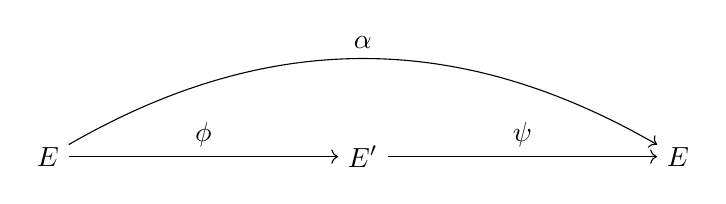
\begin{tikzpicture}
            \node (Ep) at (0, 0) {$E'$};
            \node (E1) at (-4, 0) {$E$};
            \node (E2) at (4, 0) {$E$};

            \draw [->] (E1) -- (Ep) node [midway, above] {$\phi$};
            \draw [->] (Ep) -- (E2) node [midway, above] {$\psi$};
            \draw [->] (E1) to [bend left] node [midway, above] {$\alpha$} (E2);
        \end{tikzpicture}
    \end{center}
    We assume $l \divides n$, otherwise the claim is trivial.
    However, then we have the contradiction
    \begin{align*}
        \psi((\phi \circ \tau \circ \hat{\phi})(P)) &= (\psi \circ \phi \circ \tau \circ \hat{\phi})(P) = (\alpha \circ \tau \circ \hat{\phi})(P) \\
        &= (\tau \circ \alpha \circ \hat{\phi})(P) = (\tau \circ \psi \circ [n])(P) = (\tau \circ \psi)(\IdPoint) = \IdPoint
    \end{align*}
    since $\tau \circ \alpha = \alpha \circ \tau$ ($\End(E)$ is commutative).
\end{proof}
\begin{lemma}
    Let $\O$ be a quadratic imaginary order with $p \notdivides d(\O)$ with two integral, invertible ideals $\a, \b \leq \O$.
    Let further $E$ be an Elliptic Curve with $\End(E) \cong \O$.
    Identifying $\End(E_\a)$ with $\O$ by the canonical isomorphism $\Phi_{E, \a}: \End(E) \overset{\sim}{\longrightarrow} \End(E_\a)$, we have
    \begin{equation*}
        E_{\a\b} \cong (E_\a)_\b \quad \text{and} \quad \phi_{E, \a\b} = \phi_{E_\a, \b} \circ \phi_{E, \a}
    \end{equation*}
\end{lemma}
\begin{proof}
    First, we show that $\Phi_{E, \a}(\pi_E) = \pi_{E_\a}$ and so we can write $\pi \in \O$ for the unique element mapping to the Frobenius in $\End(E)$ resp. $\End(E_\a)$.
    We have that
    \begin{equation*}
        \Phi_{E, \a}(\pi_E) = \frac 1 {\deg(\phi_{E, \a})} \phi_{E, \a} \circ \pi_E \circ \hat{\phi}_{E, \a}
    \end{equation*}
    and so
    \begin{equation*}
        \phi_{E, \a} \circ \hat{\phi}_{E, \a} \circ \Phi_{E, \a}(\pi_E) = \phi_{E, \a} \circ \pi_E \circ \hat{\phi}_{E, \a}
    \end{equation*}
    Counting separability degrees on both sides shows that $\Phi_{E, \a}(\pi_E)$ is purely inseparable, thus must be the Frobenius $\pi_{E_\a}$.
    
    Now write $\a = \tilde{\a} (p, \pi)^r$ and $\b = \tilde{\b} (p, \pi)^s$.
    It is now the case that
    \begin{equation*}
        \phi_{E, \a\b} = \phi_{E, \tilde{\a} \tilde{\b}}^{(p^{r + s})}
    \end{equation*}
    and
    \begin{equation*}
        \phi_{E_\a, \b} \circ \phi_{E, \a} = (\phi_{E_\a, \tilde{\b}} \circ \pi_r \circ \phi_{E, \tilde{\a}})^{(p^s)} = (\phi_{E_\a, \tilde{\b}} \circ \phi)^{(p^r)} = (\phi_{E_\a, \tilde{\b}}^{(q/p^r)} \circ \phi_{E, \tilde{\a}})^{(p^{r + s})}
    \end{equation*}
    where $\pi_r: E_{\tilde{\a}} \to E_{\tilde{\a}}^{(p^r)}$ is the $p^r$-th power Frobenius and $\phi_{E_\a, \tilde{\b}}$ is defined over $\F_q$.
    Note that $\phi_{E_\a, \tilde{\b}}$ is the separable isogeny with kernel $E_\a[\tilde{\b}]$ and thus $\phi_{E_\a, \tilde{\b}}^{(q/p^r)}$ is the separable isogeny with kernel $E_{\a}^{(q/p^r)}[\tilde{\b}] = E_{\tilde{\a}}[\tilde{\b}]$.
    In other words, find
    \begin{equation*}
        \phi_{E_\a, \tilde{\b}}^{(q/p^r)} = \phi_{E_{\tilde{\a}}, \tilde{\b}}
    \end{equation*}
    and so it suffices to show the claim in the case that $\a = \tilde{\a}$, $\b = \tilde{\b}$ are integral, invertible ideals coprime to $(p, \pi)$.

    Having reduced everything to the separable case, it now suffices to show that $\ker(\phi_{E_\a, \b} \circ \phi_{E, \a}) = E[\a\b]$.
    For simplicity of notation, write $\phi = \phi_{E, \a}$ and $\psi = \phi_{E_\a, \b}$.
    Hence, we want to show that $\ker(\psi \circ \phi) = E[\a\b]$.

    The crucial point here is that our isomorphism $\End(E) \cong \End(E_\a)$ is given by $\Phi$.
    Since the identification of $\End(E)$ and $\End(E_\a)$ would hide this, we will be explicit in this part and write
    \begin{align*}
        i: \O \to \End(E) \quad \text{and} \quad i': \O \to \End(E')
    \end{align*}
    for the isomorphisms.
    Note that $\Phi \circ i = i'$.
    We have
    \begin{align*}
        \ker(\psi \circ \phi) =& \phi^{-1}(\ker\psi) = \phi^{-1}(E'[\mathfrak{a}]) = \phi^{-1}\Bigl( \bigcap_{\tau \in \mathfrak{a}} \ker(i'(\tau)) \Bigr) \\
        =& \bigcap_{\tau \in \mathfrak{a}} \phi^{-1}(\ker(i'(\tau))) = \bigcap_{\tau \in \mathfrak{a}} \ker(i'(\tau) \circ \phi) \overset{(*)}{=} \bigcap_{\tau \in \mathfrak{a}} \ker(\phi \circ i(\tau)) \\
        =& \bigcap_{\tau \in \mathfrak{a}} i(\tau)^{-1}(\ker\phi) = \bigcap_{\tau \in \mathfrak{a}} i(\tau)^{-1}(E[\mathfrak{b}]) = \bigcap_{\tau \in \mathfrak{a}, \ \rho \in \mathfrak{b}} i(\tau)^{-1}(\ker(i(\rho))) \\
        =& \bigcap_{\tau \in \mathfrak{a}, \ \rho \in \mathfrak{b}} \ker(\underbrace{i(\rho) \circ i(\tau)}_{\mathclap{= i(\rho\tau) \in i(\a\b)}}) = E[\mathfrak{b}\mathfrak{a}]
    \end{align*}
    The equality at $(*)$ holds, since
    \begin{equation*}
        i'(\tau) = (\Phi_* \circ i)(\tau) = \frac 1 {\deg(\phi)} \phi \circ i(\tau) \circ \hat{\phi} \qedhere
    \end{equation*}
\end{proof}
\begin{lemma}
    \label{prop:inseparable_iff_frobenius_ideal}
    Let $E$ be an ordinary curve and $\alpha \in \End(E)$.
    Then $\alpha$ inseparable if and only if $\alpha \in (p, \pi)$.
\end{lemma}
\begin{proof}
    First, consider
    \begin{equation*}
        \b := \{ \beta \in \End(E) \ | \ \text{$\beta$ inseparable} \}
    \end{equation*}
    This is an ideal, as for two inseparable $\beta_1, \beta_2 \in \End(E)$ have that they factor as
    \begin{center}
        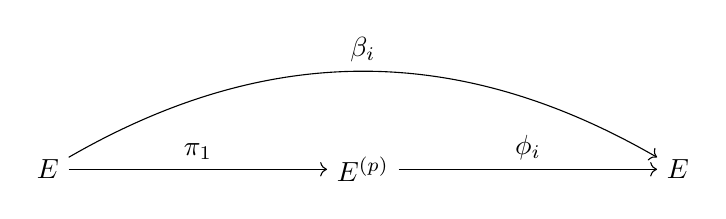
\begin{tikzpicture}
            \node (Ep) at (0, 0) {$E^{(p)}$};
            \node (E1) at (-4, 0) {$E$};
            \node (E2) at (4, 0) {$E$};

            \draw [->] (E1) -- (Ep) node [midway, above] {$\pi_1$};
            \draw [->] (Ep) -- (E2) node [midway, above] {$\phi_i$};
            \draw [->] (E1) to [bend left] node [midway, above] {$\beta_i$} (E2);
        \end{tikzpicture}
    \end{center}
    with the $p$-th power Frobenius $\pi_1$.
    Now $\beta_1 + \beta_2 = (\phi_1 + \phi_2) \circ \pi_1$ is inseparable, and clearly $\beta \gamma$ is inseparable for $\beta \in \b$ and $\gamma \in \End(E)$ (just compare separability degrees).

    Furthermore, $p$ and $\pi$ are inseparable, so $(p, \pi) \subseteq \b$.
    Note that in the imaginary quadratic order $\End(E)$, every prime ideal is maximal.
    Since $\Norm((p, \pi)) = p \perp d(\End(E))$, Prop.~\ref{prop:coprime_ideals_order} shows that $(p, \pi)$ is prime, and thus $(p, \pi) = \b$ (clearly, $\b \neq \End(E)$).
\end{proof}
\begin{lemma}
    Let $E$ be an ordinary curve and $\a, \b \leq \End(E)$ two integral, invertible ideals.
    Then $E_\a \cong E_\b$ if and only if $[\a] = [\b] \in \Cl(\End(E))$ are in the same ideal class.
\end{lemma}
\begin{proof}
    First, we show the direction $\Leftarrow$.
    By assumption, there are $\alpha, \beta \in \O$ such that $\alpha\a = \beta\b$.
    Thus $E_{\alpha\a} = E_{\beta\b}$ and it suffices to show that for any Elliptic Curve $E$ and $\alpha \in \End(E)$, have $E_{(\alpha)} \cong E$.

    Write $(\alpha) = (p, \pi)^r \a$ and assume that $E$ is defined over $\F_{p^s}$.
    Then $(\alpha)(p)^{\lceil r/s \rceil s - r} = (\pi)^{\lceil r/s \rceil}(\alpha')$ since $(p) = (p, \pi)(p, \pi - t)$ and $(p, \pi)^s = (\pi)$ by an easy computation.
    Furthermore, $\alpha' \notin (p, \pi)$.
    Now note that for any curve $E$, have $E_{(\pi)} = E^{(p^s)} \cong E$ and $E_{(p)} \cong E$, where the latter holds, since in the ordinary case, $p$ factors as
    \begin{center}
        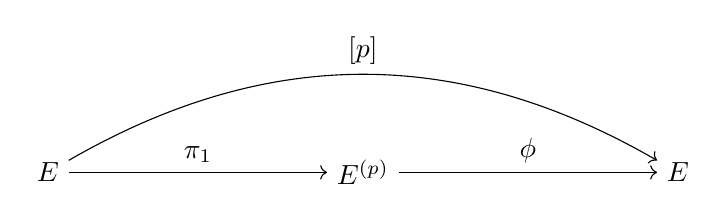
\begin{tikzpicture}
            \node (Ep) at (0, 0) {$E^{(p)}$};
            \node (E1) at (-4, 0) {$E$};
            \node (E2) at (4, 0) {$E$};

            \draw [->] (E1) -- (Ep) node [midway, above] {$\pi_1$};
            \draw [->] (Ep) -- (E2) node [midway, above] {$\phi$};
            \draw [->] (E1) to [bend left] node [midway, above] {$[p]$} (E2);
        \end{tikzpicture}
    \end{center}
    with the $p$-th power Frobenius $\pi_1$ and $\phi$ is separable with $\ker(\phi) = E[p] = \ker([p]) \cap \ker(\pi - t)$.
    Thus we see that $E_{(\alpha)} \cong E_{(\alpha')}$ and can assume wlog that $\alpha = \alpha' \notin (p, \pi)$.

    By Lemma~\ref{prop:inseparable_iff_frobenius_ideal}, we now see that $\alpha$ is separable, and so clearly $\ker(\alpha) = E[(\alpha)]$.
    Since $\alpha: E \to E$ is the separable isogeny on $E$ with kernel $E[(\alpha)]$, we see that $E_{(\alpha)} = E/E[(\alpha)] \cong E$.

    Now we consider the other direction $\Rightarrow$.
    Again, write $\a = \tilde{\a}(p, \pi)^r$ and assume that $E$ is defined over $\F_{p^s}$.
    Then we have as before that $\a (p)^{\lceil r/s \rceil s - r} = (\pi)^{\lceil r/s \rceil} \a'$ for the ideal $\a' = \tilde{\a} (p, \pi - t)^{\lceil r/s \rceil s - r}$.
    Now clearly $[\a] = [\a']$ are in the same ideal class and $\a' \perp (p, \pi)$.
    Furthermore, by the direction $\Leftarrow$, have $E_\a \cong E_{\a'}$.
    Doing the same with $\b$, we can assume wlog that $\a = \a'$ and $\b = \b'$ are ideals coprime to $(p, \pi)$.

    Therefore, the isogenies $\phi_{E, \a}$ and $\phi_{E, \b}$ are separable.
    Write $E' := E_\a = E_\b$.
    Choose $N > 0$ such that $[N]^{-1}(E[\a]) \supseteq E[\b]$.
    Now the isogeny $[N] \circ \phi_{E, \a}$ factors through $\phi_{E, \b}$, i.e. we get a commutative diagram
    \begin{center}
        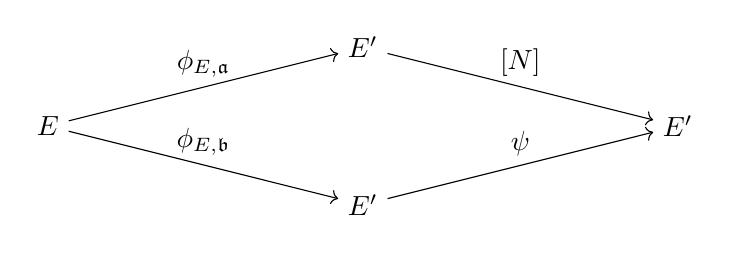
\begin{tikzpicture}
            \node (E1) at (0, 1) {$E'$};
            \node (E2) at (0, -1) {$E'$};
            \node (E0) at (-4, 0) {$E$};
            \node (E3) at (4, 0) {$E'$};

            \draw [->] (E0) -- (E1) node [midway, above] {$\phi_{E, \a}$};
            \draw [->] (E0) -- (E2) node [midway, above] {$\phi_{E, \b}$};
            \draw [->] (E1) -- (E3) node [midway, above] {$[N]$};
            \draw [->] (E2) -- (E3) node [midway, above] {$\psi$};
        \end{tikzpicture}
    \end{center}
    for some endomorphism $\psi: E' \to E'$.
    Clearly the isogenies $[N]$ and $\psi$ are given by the ideals $(N)$ resp. $(\psi)$, and so we find
    \begin{equation*}
        (N)\a = (\psi)\b
    \end{equation*}
    and the claim follows.
\end{proof}
\begin{theorem}
    Let $\O$ be an imaginary quadratic order with $p \notdivides d(\O)$ and denote by $\Ell(\O)$ the set of isomorphism classes of all Elliptic Curves $E$ over $\bar{\F}_p$ with $\End(E) \cong \O$.
    Then there is a free and transitive group action
    \begin{equation*}
        \Cl(\O) \times \Ell(\O) \to \Ell(\O), \quad ([\a], E) \mapsto E_\a
    \end{equation*}
    where $\a$ is an integral, invertible ideal representative of the ideal class $[\a]$.
\end{theorem}
\begin{proof}
    Well-definedness and freeness follow from all the previous lemmas.
\end{proof}
A similar class group action exists in many other cases, since it is really founded in the theory of abelian varieties, see \cite{class_group_action_waterhouse}.
Notable examples are the CSIDH class group action for supersingular curves defined over $\F_p$ (see \cite{csidh}), its generalization to so-called oriented curves (see \cite{osidh}), and the very classical class group action of Elliptic Curves with complex multiplication (over $\C$).
More concretely, if we consider an order $\O$ in a quadratic imaginary number field and write $\Ell(\O)$ for the set of (isomorphism classes of) curves over $\C$ with endomorphism ring $\O$ (these are said to have \emph{complex multiplication}), then there is a free and transitive class group action
\begin{equation*}
    \Cl(\O) \times \Ell(\O) \to \Ell(\O), \quad ([\a], E) \to E/E[\a]
\end{equation*}
where we choose $\a$ to be an integral ideal representative of $[\a]$.
Note that for ideals $\a \perp (p, \pi)$, this is analogous to our action defined above.
However, since the Frobenius has trivial kernel, one needs some addition in the finite field case.

Note that one can still keep the simpler definition
\begin{equation*}
    \Cl(\O) \times \Ell(\O) \to \Ell(\O), \quad ([\a], E) \to E/E[\a]
\end{equation*}
also in the finite field case, if we require $\a$ to be an (integral) ideal representative of $[\a]$ that is coprime to $(p, \pi)$.
Clearly, every ideal class has such a representative, since we can multiply with the principal ideal $(p) = (p, \pi)(p, \pi - t)$ and divide out the principal ideal $(\pi) = (p, \pi)^s$.
However, some sources do not explicitly mention that $\a$ must be chosen coprime to $(p, \pi)$, which caused me some confusion.

\subsection{Vulcanoes}

\section{Supersingular isogeny graphs}

\section{Generating supersingular curves}

\end{document}
